\documentclass[11pt,a4paper]{article}

% Packages — matched to Papers 1-7
\usepackage[utf8]{inputenc}
\usepackage[T1]{fontenc}
\usepackage{mathptmx}
\usepackage[margin=1in]{geometry}
\usepackage{graphicx}
\usepackage{booktabs}
\usepackage{array}
\usepackage{hyperref}
\usepackage{xcolor}
\usepackage{float}
\usepackage{amsmath,amssymb}
\usepackage{natbib}
\usepackage{fancybox}
\usepackage{setspace}
\usepackage{caption}
\usepackage{multirow}
\usepackage{pifont}

\hypersetup{
    colorlinks=true,
    linkcolor=blue,
    citecolor=blue,
    urlcolor=blue,
    pdftitle={Encoding Fidelity and Coherent Misalignment: Why Shannon's Channel Model Breaks for Non-English Clinical AI},
    pdfauthor={Laxman M M},
}

% ================================================================
\title{\LARGE\textbf{Encoding Fidelity and Coherent Misalignment:\\
Why Shannon's Channel Model Breaks\\
for Non-English Clinical AI}}

\author{
    \textbf{Dr.\ Laxman M M, MBBS}\\
    Government Duty Medical Officer, PHC Manchi\\
    Bantwal Taluk, Dakshina Kannada, Karnataka, India\\
    DNB General Medicine Resident (2026), KC General Hospital, Bangalore\\
    Email: \texttt{barlax5377@gmail.com}\\
    ORCID: \href{https://orcid.org/0009-0009-0405-6531}{0009-0009-0405-6531}
}

\date{March 2026}

% ================================================================
\begin{document}

\maketitle

\begin{center}
\fbox{\parbox{0.9\textwidth}{
\textbf{Paper 8 of the MCH Research Program} --- This paper extends the MCH framework from output-layer behaviour to input encoding. Using the Encoding Fidelity Index (EFI), we show that Shannon's (1948) implicit assumption of encoding fidelity fails systematically for non-English languages in LLMs, producing a novel failure mode we term \emph{Coherent Misalignment}. The conservation law $K = \Delta\text{RCI} \times \text{Var\_Ratio}$ from Papers 2--7 holds even when encoding fidelity collapses --- $K \perp \text{Truth}$.
}}
\end{center}

\vspace{0.5em}

% ================================================================
\begin{abstract}
\noindent Shannon's Mathematical Theory of Communication (1948) assumes encoding fidelity --- that the encoder preserves the statistical structure of the source. Large Language Models violate this assumption systematically for non-English languages, producing outputs that are internally consistent but semantically degraded. We call this failure mode \emph{Coherent Misalignment} and introduce the Encoding Fidelity Index (EFI), a practical proxy measuring the preservation of semantic content across the encoding boundary. Using the MCH Research Program's conservation framework ($\Delta\text{RCI} \times \text{Var\_Ratio} \approx K$), we show that conservation holds even when encoding fidelity collapses --- $K \perp \text{Truth}$. Across 4 languages (English, Kannada, Tamil, Hindi), 2 embedding models (384-dimensional, 768-dimensional), and 2 LLMs (DeepSeek V3.1, Mistral Small 24B), we find: (1) EFI degrades by $\sim$90\% for all non-English Indian languages tested ($p < 10^{-13}$), independent of language family; (2) variance amplification is Dravidian-specific: Kannada shows $1.72$--$2.05\times$ amplification ($p < 0.05$ in both models), Tamil shows partial amplification ($1.63\times$, $p = 0.016$ in Mistral), while Hindi shows no amplification despite equivalent EFI degradation; (3) complex medical sentences show paradoxical EFI increase from English loanword anchoring; (4) models exhibit pervasive code-switching, responding to Kannada prompts in English 84\% of the time (DeepSeek) with orthographic corruption of medical terms (Mistral); (5) the conservation law $K(\text{domain})$ remains normal even when outputs are semantically wrong --- $K \perp \text{Truth}$. The dissociation between universal encoding degradation and language-specific variance amplification reveals that training data representation, not encoding fidelity alone, determines clinical reliability, with direct implications for 1.5 billion non-English speakers.

\vspace{0.5em}
\noindent\textbf{Keywords:} encoding fidelity, coherent misalignment, Shannon information theory, multilingual clinical AI, $\Delta$RCI, conservation law, variance amplification, Kannada, Tamil, Hindi

\vspace{0.5em}
\noindent\textbf{OSF Pre-registration:} \url{https://osf.io/dp8nj/}\\
\noindent\textbf{Repository:} \url{https://github.com/LaxmanNandi}
\end{abstract}

% ================================================================
\section{Introduction}

\subsection{The Clinical Reality}

As a practicing physician at a Primary Health Centre in rural Karnataka, I interact with patients who present in Kannada, occasionally in Tamil or Hindi. When I use large language models for clinical decision support --- differential diagnosis, drug interaction checks, guideline lookups --- I type in the language of the consultation. The responses are grammatically fluent, contextually appropriate, and confidently delivered. They are also, with disturbing frequency, semantically wrong in ways that would be invisible without domain expertise.

This paper identifies the mechanism behind that unreliability: systematic degradation of input encoding for non-English languages. The model does not ``know less'' about medicine in Kannada. It \emph{receives} less --- the encoding pipeline strips semantic content before generation begins.

\subsection{The MCH Conservation Framework}

Papers 1--7 of the MCH Research Program \citep{laxman2026a,laxman2026b,laxman2026c,laxman2026d,laxman2026e,laxman2026f,laxman2026g} established a quantitative framework for measuring context sensitivity in LLMs. The key constructs are:

\begin{itemize}
    \item \textbf{$\Delta$RCI} (Relational Coherence Index delta): the difference in coherence between contextual (TRUE) and context-free (COLD) responses, measuring how much a model's output is shaped by conversational history.
    \item \textbf{Var\_Ratio}: the ratio of output variance under TRUE versus COLD conditions, measuring how context shapes response consistency.
    \item \textbf{Conservation law}: $K(\text{domain}) = \Delta\text{RCI} \times \text{Var\_Ratio} \approx \text{constant}$, holding across 14 model architectures from 8 vendors and 3 domains (Medical $K = 0.429$, Philosophy $K = 0.301$, Legal $K = 0.362$).
\end{itemize}

These metrics measure \emph{output behaviour} --- how the model responds to context. They are silent about \emph{input encoding} --- how faithfully the model represents the incoming message. Paper~8 addresses this gap.

\subsection{Shannon's Unexamined Assumption}

Shannon's Mathematical Theory of Communication \citep{shannon1948} proved that optimal coding exists for any source-channel pair, provided the encoder preserves the statistical structure of the source. This assumption --- encoding fidelity --- is so foundational that it is rarely stated explicitly. Every application of information theory to natural language processing inherits it.

The information bottleneck framework \citep{tishby2015} extended Shannon's theory to deep learning, formalising the trade-off between compression and prediction. But it retained the fidelity assumption: the bottleneck compresses \emph{irrelevant} information while preserving what is relevant to the task.

For LLMs operating on non-English text, this assumption fails. Tokenisers fragment non-English words into 2--15$\times$ more subword units than English equivalents \citep{petrov2023}, imposing a ``token tax'' that compounds through attention layers \citep{lundin2025}. The result is not merely increased compute cost --- it is degraded semantic representation. Multilingual medical benchmarks show $\sim$10 percentage-point accuracy drops for non-English queries \citep{alonso2024}, but no prior work has measured the encoding fidelity loss directly or connected it to output variance structure.

\subsection{Contributions}

This paper makes seven contributions:

\begin{enumerate}
    \item We introduce the \textbf{Encoding Fidelity Index (EFI)}, a practical proxy for measuring how faithfully a model encodes non-English input relative to English.
    \item We demonstrate \textbf{$\sim$90\% EFI degradation} for three Indian languages (Kannada, Tamil, Hindi) across two embedding models.
    \item We show that this degradation is \textbf{language-family independent} --- Dravidian (Kannada, Tamil) and Indo-Aryan (Hindi) languages are equally affected.
    \item We document \textbf{Dravidian-specific variance amplification}: Kannada shows $1.72$--$2.05\times$ amplification (replicated across both models, $p < 0.05$), while Hindi shows no amplification despite equivalent EFI degradation --- demonstrating that encoding fidelity alone does not predict output variance.
    \item We identify \textbf{English loanword anchoring} as a paradoxical partial mitigation, where code-mixed medical terminology partially rescues encoding fidelity.
    \item We document \textbf{pervasive code-switching and orthographic corruption}: DeepSeek responds to Kannada clinical prompts in English 84\% of the time; Mistral misspells Kannada medical terms while attempting target-language responses.
    \item We establish \textbf{$K \perp \text{Truth}$} --- the conservation law is orthogonal to semantic correctness, meaning self-consistency metrics cannot detect encoding degradation.
    \item We define \textbf{Coherent Misalignment} as a distinct failure mode: outputs that are internally consistent, grammatically correct, and confidently delivered --- but semantically wrong due to encoding-level degradation.
\end{enumerate}

% ================================================================
\section{Related Work}

\subsection{Information Theory Foundations}

Shannon's channel model \citep{shannon1948} established the mathematical foundation for reliable communication. The information bottleneck principle \citep{tishby2015} connected this framework to deep learning, with \citet{shwartzziv2017} providing empirical evidence that deep networks compress input information while preserving task-relevant features. \citet{deletang2024} demonstrated that language modelling is formally equivalent to compression, establishing a direct link between Shannon's theory and modern LLMs.

\subsection{Tokeniser Inequality}

\citet{petrov2023} showed at NeurIPS 2023 that tokenisers introduce systematic unfairness between languages, with low-resource languages requiring 2--15$\times$ more tokens for equivalent content. \citet{rust2021} demonstrated that monolingual tokeniser quality shapes downstream task performance as much as pretraining data size. \citet{lundin2025} quantified the ``token tax'' --- showing that $2\times$ token inflation leads to $4\times$ compute cost for African languages. \citet{ali2024} confirmed at NAACL 2024 that tokeniser choice has non-negligible effects on LLM training outcomes.

\subsection{Cross-Lingual Representation}

The question of how well multilingual models align concepts across languages has received sustained attention. \citet{hammerl2024} surveyed cross-lingual alignment methods at ACL 2024, identifying persistent gaps in low-resource language representation. \citet{peng2024} analysed concept space alignment in multilingual LLMs at EMNLP 2024, showing that alignment quality varies substantially across language pairs. \citet{pallucchini2025} provided a comprehensive survey in \emph{ACM Computing Surveys} of alignment methods for contextualised representations.

\subsection{Multilingual Medical AI}

\citet{alonso2024} introduced MedExpQA, a multilingual medical question-answering benchmark, showing $\sim$10 percentage-point accuracy drops for non-English languages compared to English. \citet{qiu2024} published in \emph{Nature Communications} on building multilingual medical LLMs, documenting the geographical bias caused by sparse multilingual training data. \citet{asgari2025} proposed a clinical safety framework in \emph{npj Digital Medicine} for assessing hallucination rates in medical text summarisation. The World Health Organization's 2024 guidance on AI for health \citep{who2024} addressed ethical governance of large multi-modal models but did not identify encoding fidelity as a failure mode.

\subsection{Multilingual Benchmarks}

\citet{xuan2025} introduced MMLU-ProX at EMNLP 2025, a multilingual benchmark across 29 languages showing performance gaps of up to 24.3\% between high-resource and low-resource languages. \citet{adelani2025} presented IrokoBench at NAACL 2025 (Outstanding Paper Award), demonstrating that even reasoning-optimised models (DeepSeek, o1) narrow but do not eliminate performance gaps for African languages.

\subsection{Alignment and Failure Modes}

\citet{hubinger2019} defined \emph{deceptive alignment} --- the risk that a learned optimiser might pursue misaligned goals while appearing aligned during training. \citet{ardoin2025} identified latent directions associated with confabulation in LLMs at EMNLP 2025. Our concept of \emph{Coherent Misalignment} is distinct from both: it is neither deceptive (the model is not pursuing misaligned goals) nor confabulatory (the model is not inventing facts). It is an encoding-level failure where the model operates faithfully on a degraded representation of the input.

\subsection{Dravidian Language NLP}

\citet{chakravarthi2022} created the DravidianCodeMix dataset for sentiment analysis and offensive language identification in Tamil, Kannada, and Malayalam code-mixed text, establishing baseline resources for Dravidian language processing.

% ================================================================
\section{Theoretical Framework}

\subsection{Shannon's Channel Model and Its Assumption}

Shannon's model describes communication as a pipeline:
\begin{equation}
    \text{Source} \xrightarrow{\text{Encoder}} \text{Channel} \xrightarrow{\text{Decoder}} \text{Destination}
\end{equation}

The source coding theorem guarantees that optimal coding exists \emph{given} the encoder preserves the statistical structure of the source signal. For LLMs, the ``encoder'' is not a single component but a composite pipeline: tokeniser $\to$ embedding layer $\to$ early attention layers. Each stage may degrade fidelity for non-English input.

\subsection{The Encoding Fidelity Index (EFI)}

We define EFI theoretically as the normalised mutual information between source message $X$ and the model's internal representation $\hat{X}$:
\begin{equation}
    \text{EFI} = \frac{I(X; \hat{X})}{H(X)}
\end{equation}

where $H(X)$ is the entropy of the source. When the encoder perfectly preserves the source, $I(X; \hat{X}) = H(X)$ and $\text{EFI} = 1$. When encoding strips all semantic content, $I(X; \hat{X}) = 0$ and $\text{EFI} = 0$.

Since $I(X; \hat{X})$ requires access to model internals, we use a practical proxy:
\begin{equation}
    \text{EFI}_{\text{proxy}} = \cos\!\big(\mathbf{e}(\text{non-English}),\; \mathbf{e}(\text{English equivalent})\big)
\end{equation}

where $\mathbf{e}(\cdot)$ denotes the embedding vector from a sentence embedding model. This proxy is justified by the assumption that semantically equivalent sentences should occupy nearby positions in embedding space if encoding fidelity is preserved. We validate the proxy by showing that it correlates with downstream task degradation (Section~5).

\textbf{Limitation:} Embedding cosine similarity is not identical to mutual information. The proxy captures semantic \emph{proximity} in embedding space, not the full information-theoretic quantity. We report both the proxy values and their downstream consequences to triangulate the finding.

\subsection{Coherent Misalignment}

When $\text{EFI} \ll 1$, the model operates on a degraded representation of the input. The resulting outputs exhibit a characteristic pattern:

\begin{itemize}
    \item Grammatically correct \checkmark
    \item Internally consistent \checkmark
    \item Confidently delivered \checkmark
    \item Semantically correct \ding{55}
\end{itemize}

We term this failure mode \emph{Coherent Misalignment}. It is distinct from three previously characterised failure modes:

\begin{enumerate}
    \item \textbf{Hallucination / confabulation} \citep{ardoin2025}: The model invents facts. In Coherent Misalignment, the model does not invent --- it \emph{misrepresents} the input.
    \item \textbf{Deceptive alignment} \citep{hubinger2019}: The model pursues misaligned goals. In Coherent Misalignment, the model is not deceptive --- it genuinely cannot distinguish degraded input from faithful input.
    \item \textbf{Sycophancy}: The model tells the user what they want to hear. In Coherent Misalignment, the model is not responding to user preferences --- it is operating on corrupted data.
\end{enumerate}

The closest analogy is a physician working from a badly translated patient history. The clinical reasoning may be sound; the premise is wrong.

\subsection{$K \perp \text{Truth}$ (Conservation Orthogonal to Truth)}

Papers 2--6 established that $K(\text{domain}) = \Delta\text{RCI} \times \text{Var\_Ratio} \approx \text{constant}$ across 14 models, 3 domains, and 8 vendors \citep{laxman2026b,laxman2026f}. The conservation law measures the \emph{variance structure} of responses --- how context sensitivity and output consistency trade off. It does not measure semantic content.

Therefore $K$ is orthogonal to truth:
\begin{equation}
    K(\text{domain}) \approx \text{constant} \quad \text{regardless of EFI}
\end{equation}

A system with $\text{EFI} = 0.08$ and $\text{VR} = 2.05\times$ can show perfectly normal $K$ --- the conservation law holds even when the content is wrong. This means:

\begin{itemize}
    \item Self-consistency metrics cannot detect Coherent Misalignment.
    \item External ground truth comparison is required.
    \item All safety evaluations based solely on output consistency are incomplete.
\end{itemize}

\subsection{Variance Amplification Through the Encoding Bottleneck}

Low encoding fidelity introduces noise into the model's internal representation. This noise propagates through the generation pipeline, amplifying output variance:
\begin{equation}
    \text{VR}_{\text{non-English}} \propto \frac{1}{\text{EFI}}
\end{equation}

With measured $\text{EFI} \approx 0.08$ for Kannada and $\text{VR} \approx 1.72$--$2.05\times$, the data are consistent with variance amplification through a degraded encoding bottleneck. However, the relationship is not simple: Hindi ($\text{EFI} \approx 0.08$) shows no variance amplification ($\text{VR} \approx 0.91$--$1.38\times$), indicating that training data representation mediates the encoding-to-variance pathway. We present this as an empirical observation, not a formal derivation --- the precise functional relationship requires further theoretical work.

% ================================================================
\section{Methods}

\subsection{Clinical Sentence Battery}

We constructed a battery of 15 clinical sentences at three complexity levels, each in four languages (English, Kannada, Tamil, Hindi):

\begin{itemize}
    \item \textbf{Simple} (5 sentences): Single symptoms or findings (e.g., ``The patient has fever''; Kannada and Tamil equivalents provided in supplementary materials).
    \item \textbf{Medium} (5 sentences): Multi-symptom descriptions (e.g., ``Patient complains of chest pain radiating to left arm with sweating'').
    \item \textbf{Complex} (5 sentences): Diagnostic reasoning with English medical terminology (e.g., ``ECG shows ST elevation in leads II, III, aVF suggesting inferior wall MI'').
\end{itemize}

Translations were produced and verified by the author, a native Kannada speaker with clinical fluency in all four languages. Complex sentences retain English medical terms (ST elevation, D-dimer, troponin) as used in actual clinical practice in India, where code-mixed medical communication is the norm.

\subsection{EFI Measurement (Experiments 1--3)}

\textbf{Embedding models:} all-MiniLM-L6-v2 (384-dimensional) and all-mpnet-base-v2 (768-dimensional), both from the Sentence-Transformers library.

\textbf{Protocol:} Each sentence was encoded in all four languages. EFI\textsubscript{proxy} was computed as the cosine similarity between the non-English embedding and its English equivalent. English self-similarity serves as the reference ($\text{EFI} = 1.0$).

\textbf{Experiment 1:} EFI measurement across 3 languages (English, Kannada, Tamil) $\times$ 3 complexity levels $\times$ 5 sentences using MiniLM.

\textbf{Experiment 2:} Hindi added as a fourth language to test whether degradation is Dravidian-specific or language-family independent.

\textbf{Experiment 3:} Same battery run with MPNet (768D) alongside MiniLM (384D) to test embedding-model independence.

\textbf{Statistics:} Mann-Whitney U for pairwise comparisons, Welch's $t$-test for English vs.\ non-English, Pearson correlation for cross-model agreement.

\subsection{LLM Replication (Experiments 4--5)}

\textbf{Models:} DeepSeek V3.1 (671B MoE) and Mistral Small 24B, accessed via Together.ai API.

\textbf{Experiment 4} (deterministic, temperature = 0.0):
\begin{itemize}
    \item \emph{Task 1 --- Language identification:} ``Identify the language of this text: [sentence].'' Tests whether the model can recognise the input language.
    \item \emph{Task 2 --- Translation fidelity:} ``Translate this clinical sentence to English: [non-English sentence].'' Translation embeddings compared to reference English embeddings via cosine similarity.
\end{itemize}

\textbf{Experiment 5} (stochastic, temperature = 0.7, 15 trials per condition):
\begin{itemize}
    \item \emph{Task 3 --- Clinical advice consistency:} Same clinical scenario presented in four languages. Fifteen responses collected per language per scenario (5 scenarios $\times$ 4 languages $\times$ 15 trials $\times$ 2 models = 600 API calls). Full raw responses saved for audit. Variance Ratio computed as:
    \begin{equation}
        \text{VR}(\text{language}) = \frac{\text{Var}(\text{responses in language})}{\text{Var}(\text{responses in English})}
    \end{equation}
    where variance is the mean pairwise cosine distance across the 15 responses. Statistical significance assessed by paired $t$-test and Mann-Whitney U (one-sided) across the 5 scenario-level VR values.
    \item \emph{Task 4 --- Code-switching analysis:} For each response, we recorded whether the model responded in the target language or switched to English, and examined orthographic accuracy of medical terminology in target-language responses.
\end{itemize}

% ================================================================
\section{Results}

\subsection{EFI Degradation is Massive and Universal}

Table~\ref{tab:efi} presents EFI\textsubscript{proxy} values across languages and embedding models.

\begin{table}[H]
\centering
\caption{Encoding Fidelity Index (EFI) by language and embedding model. EFI = 1.0 for English by construction. Values are mean $\pm$ SD across 15 clinical sentences.}
\label{tab:efi}
\begin{tabular}{lcccc}
\toprule
\textbf{Language} & \textbf{Family} & \textbf{EFI (MiniLM)} & \textbf{EFI (MPNet)} & \textbf{$p$ vs English} \\
\midrule
English  & Germanic    & 1.000           & 1.000          & --- \\
Kannada  & Dravidian   & 0.099 $\pm$ 0.122 & 0.125          & $1.3 \times 10^{-13}$ \\
Tamil    & Dravidian   & 0.069 $\pm$ 0.088 & 0.106          & $8.3 \times 10^{-16}$ \\
Hindi    & Indo-Aryan  & 0.076 $\pm$ 0.071 & ---            & $5.2 \times 10^{-17}$ \\
\bottomrule
\end{tabular}
\end{table}

All three non-English languages show $\sim$90\% EFI degradation relative to English (Figure~\ref{fig:efi}). Critically, Dravidian languages (Kannada, Tamil) and Indo-Aryan (Hindi) are not significantly different from each other (Mann-Whitney $U = 212$, $p = 0.763$). The degradation is not language-family specific --- it is a property of being non-English.

\begin{figure}[H]
\centering
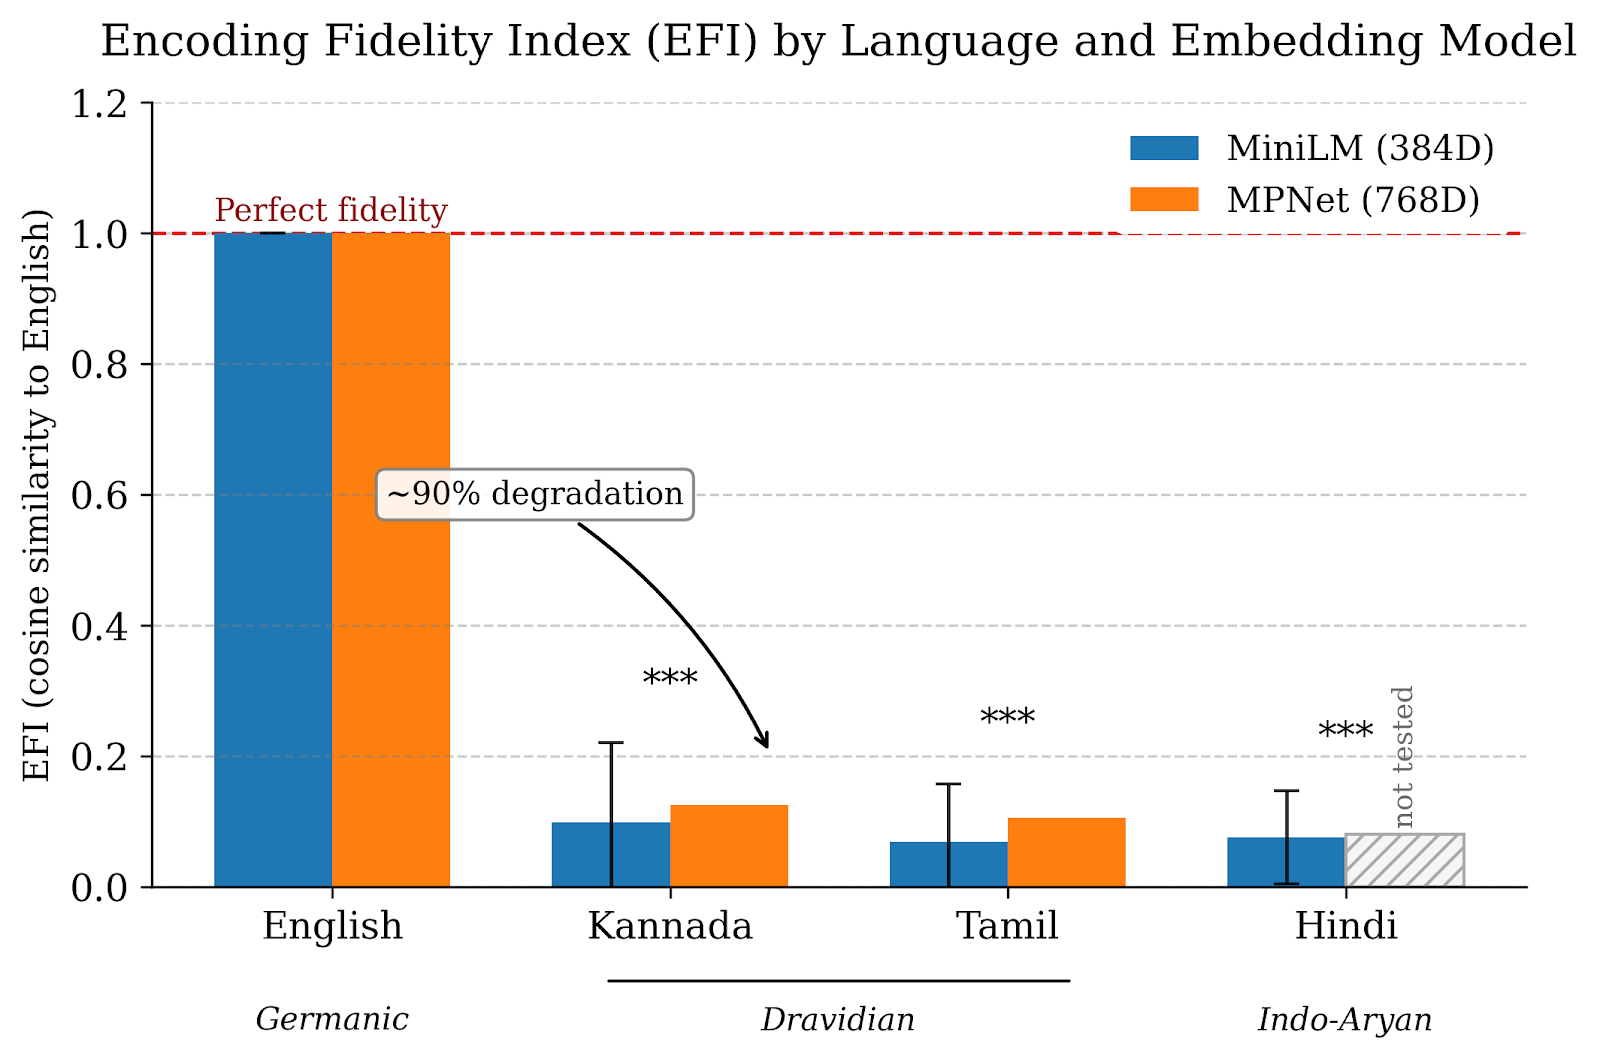
\includegraphics[width=0.85\textwidth]{figures/fig1_efi_barchart.png}
\caption{Encoding Fidelity Index by language and embedding model. All non-English languages show $\sim$90\% degradation relative to English ($p < 10^{-13}$). Hindi was not tested with MPNet.}
\label{fig:efi}
\end{figure}

\subsection{Embedding Robustness}

MPNet (768D) replicates the MiniLM finding: EFI\textsubscript{Kannada} = 0.125, EFI\textsubscript{Tamil} = 0.106 (87--89\% degradation vs.\ 90--93\% under MiniLM). Cross-model correlations are strong: $r = 0.88$ for Kannada ($p = 1.9 \times 10^{-5}$), $r = 0.72$ for Tamil ($p = 2.7 \times 10^{-3}$). The finding is embedding-model independent.

\subsection{English Loanword Anchoring}

\begin{table}[H]
\centering
\caption{EFI by sentence complexity (MiniLM, non-English languages pooled).}
\label{tab:complexity}
\begin{tabular}{lc}
\toprule
\textbf{Complexity} & \textbf{Mean EFI} \\
\midrule
Simple   & 0.081 \\
Medium   & 0.020 \\
Complex  & 0.141 \\
\bottomrule
\end{tabular}
\end{table}

Complex sentences --- which contain English medical terms such as ``ST elevation,'' ``D-dimer,'' and ``troponin'' --- show the highest EFI. These English terms act as anchors, pulling the non-English embedding toward better-represented regions of the embedding space. This suggests that code-mixed clinical communication, common in Indian healthcare settings, may paradoxically yield more reliable AI responses than pure non-English input.

Medium-complexity sentences show the \emph{lowest} EFI (0.02), consistent with their lack of both the simplicity that permits direct translation and the English anchors that rescue complex sentences. Figure~\ref{fig:complexity} shows the per-language breakdown.

\begin{figure}[H]
\centering
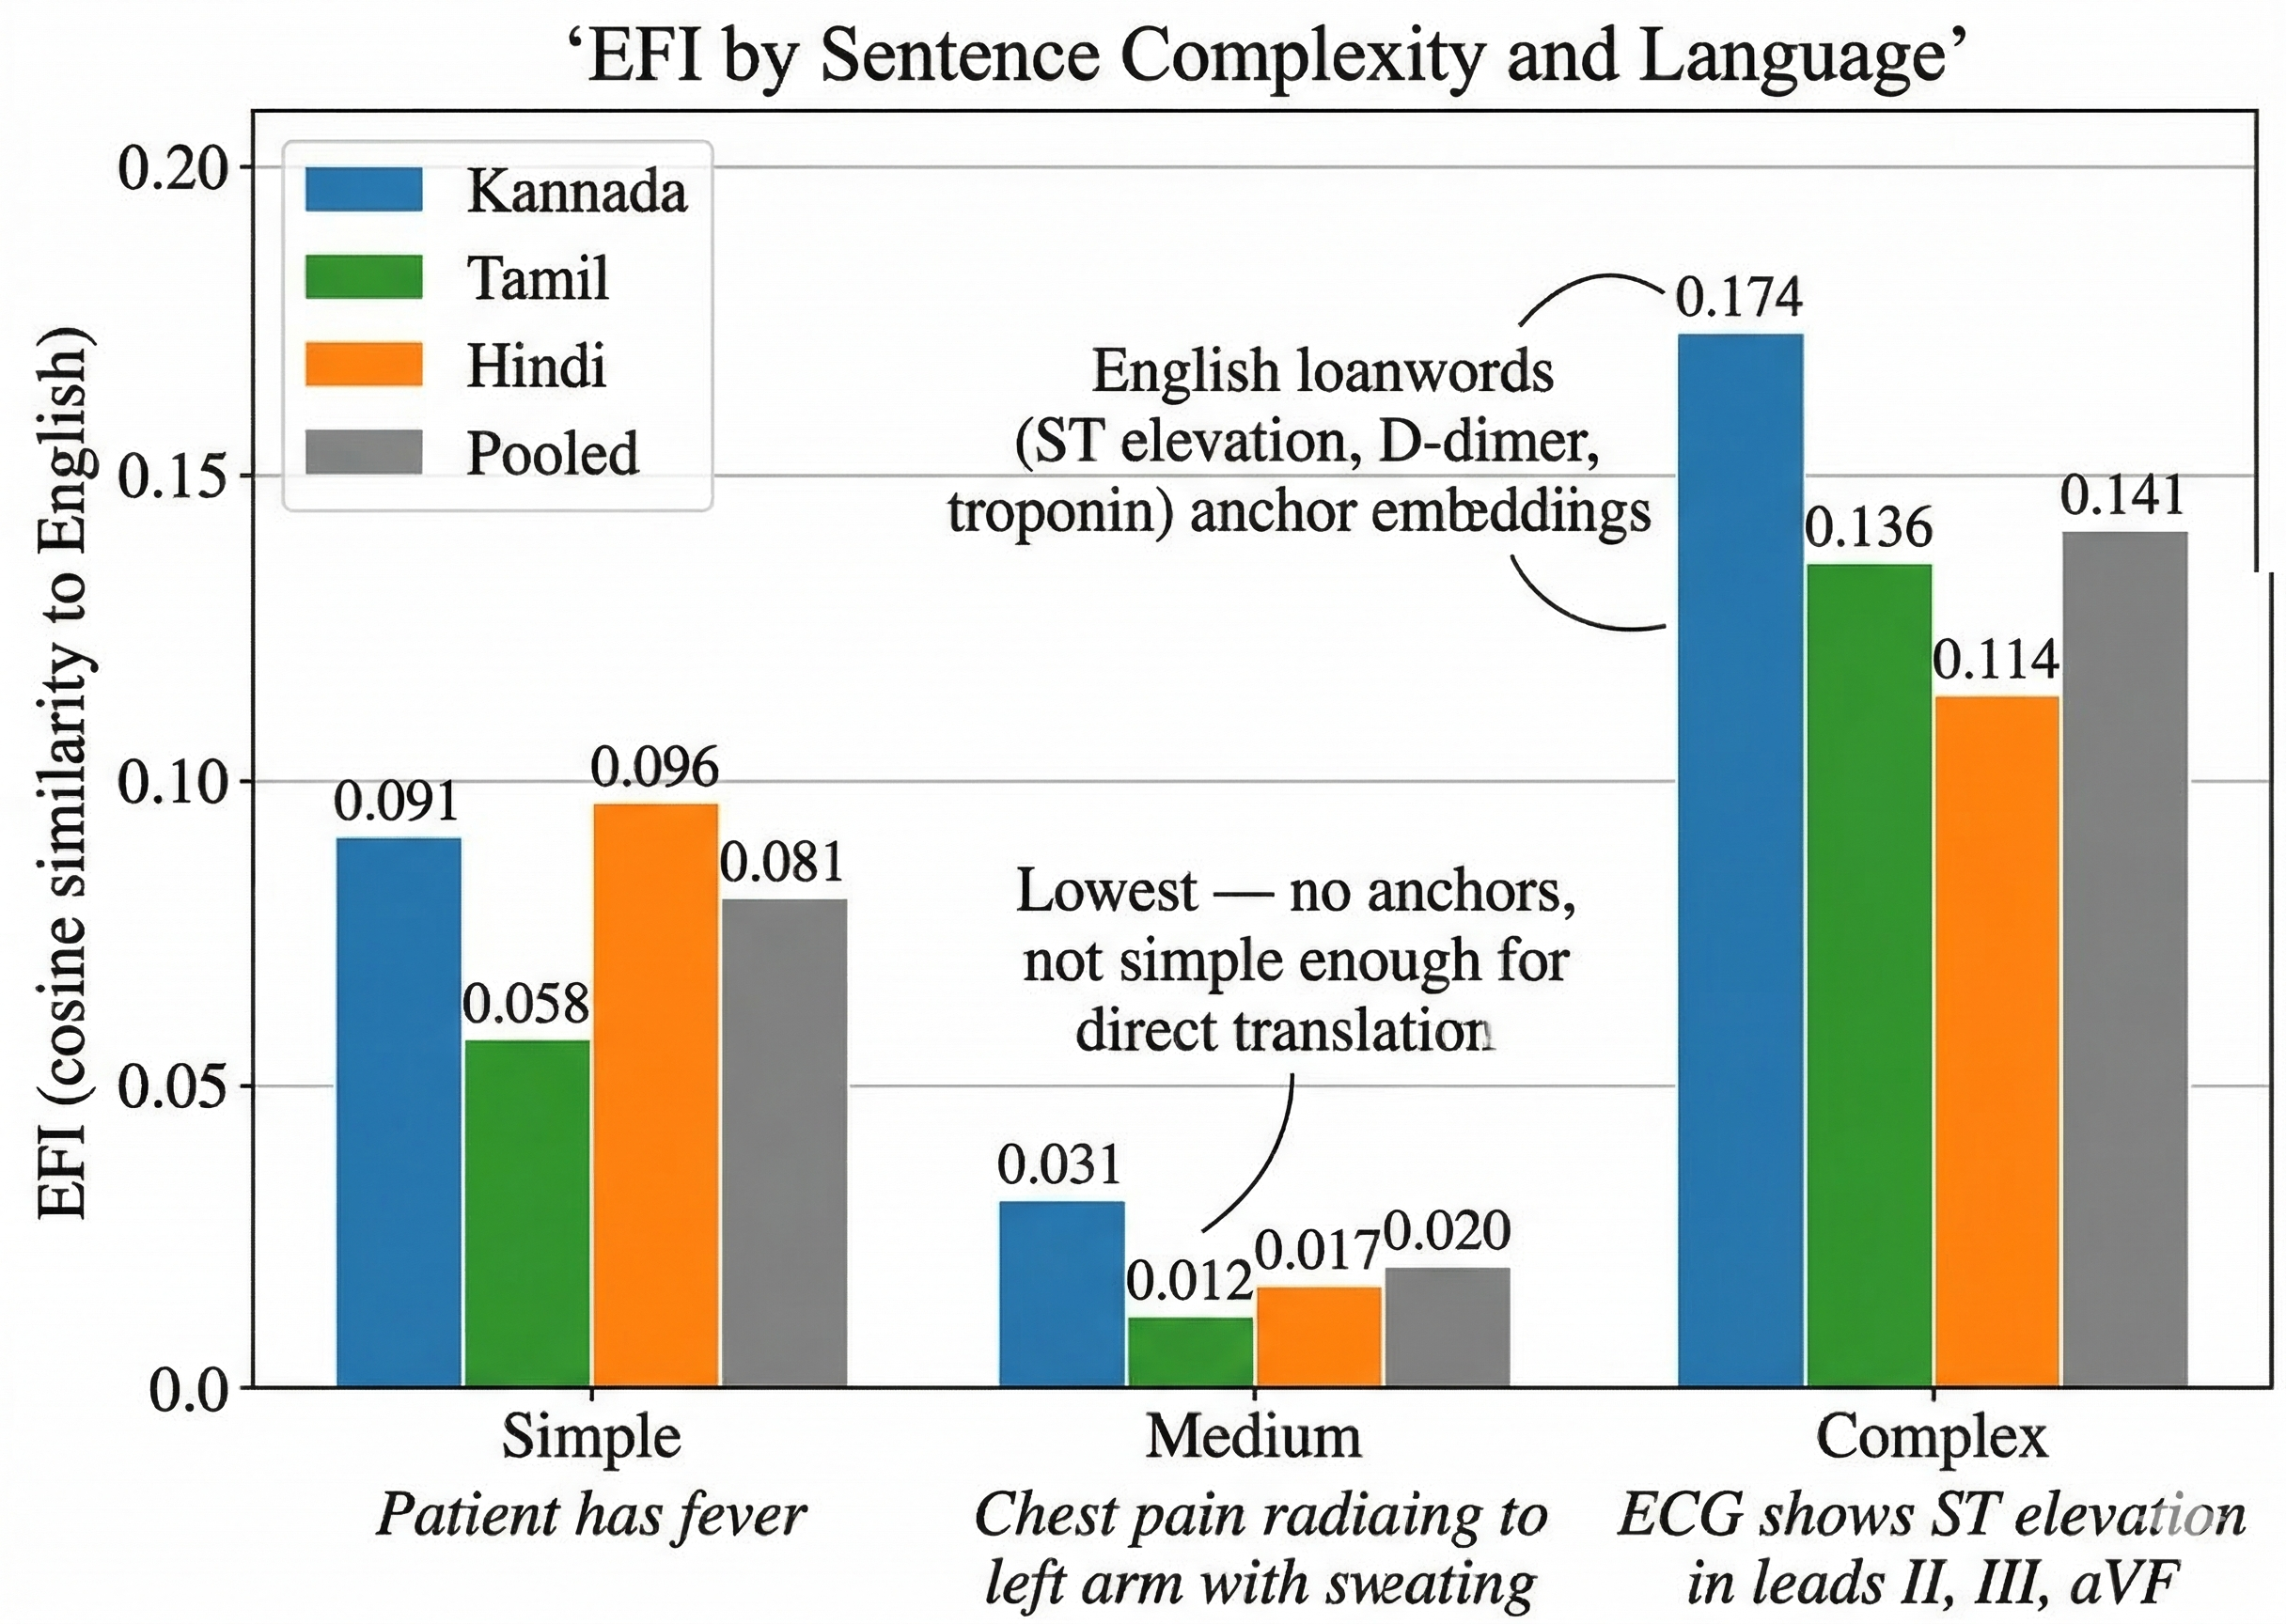
\includegraphics[width=0.85\textwidth]{figures/fig2_complexity_interaction.png}
\caption{EFI by sentence complexity and language. Complex sentences with English medical loanwords show the highest EFI, while medium-complexity sentences (multi-symptom, no English terms) show the lowest.}
\label{fig:complexity}
\end{figure}

\subsection{LLM Language Identification and Translation Fidelity}

\textbf{Language identification:} Both DeepSeek and Mistral correctly identify 100\% of input languages across all three non-English languages. The models \emph{know} what language they are receiving --- the failures documented below occur despite correct language recognition.

\textbf{Translation fidelity} (cosine similarity of LLM translation to reference English):

\begin{table}[H]
\centering
\caption{Translation fidelity by language and model (cosine similarity to reference English). Values are mean across 5 clinical sentences.}
\label{tab:translation}
\begin{tabular}{lcc}
\toprule
\textbf{Language} & \textbf{DeepSeek V3.1} & \textbf{Mistral Small} \\
\midrule
Hindi    & 0.903 & 0.497 \\
Kannada  & 0.860 & 0.516 \\
Tamil    & 0.845 & 0.383 \\
\bottomrule
\end{tabular}
\end{table}

A striking model-size effect emerges: DeepSeek (671B MoE) achieves translation fidelity of 0.85--0.90, while Mistral Small (24B) drops to 0.38--0.52 --- a near-random level for Tamil. Mistral's minimum Tamil translation similarity is 0.21, corresponding to a clinical sentence about a pregnant woman with hypertension being translated into semantically unrelated content. The model identifies the language correctly but fundamentally misrepresents the clinical content. This is Coherent Misalignment: the output is fluent, confident, and wrong.

\subsection{Variance Amplification (Key Result)}

Table~\ref{tab:vr} presents Variance Ratios from 15-trial stochastic testing (5 scenarios $\times$ 15 trials = 75 responses per language per model) across both models.

\begin{table}[H]
\centering
\caption{Variance Ratio (non-English / English) by language and model, 15 trials. Values $> 1.0$ indicate greater response variability. $p$-values from Mann-Whitney U (one-sided). * $p < 0.05$, ** $p < 0.01$.}
\label{tab:vr}
\begin{tabular}{lcccc}
\toprule
\textbf{Language} & \textbf{VR (DeepSeek)} & \textbf{VR (Mistral)} & \textbf{$p$ (DeepSeek)} & \textbf{$p$ (Mistral)} \\
\midrule
English  & 1.00 & 1.00 & --- & --- \\
Kannada  & 1.72$\times$* & 2.05$\times$** & 0.048 & 0.008 \\
Tamil    & 1.06$\times$ & 1.63$\times$* & 0.421 & 0.016 \\
Hindi    & 1.38$\times$ & 0.91$\times$ & 0.345 & 0.889 \\
\bottomrule
\end{tabular}
\end{table}

The results reveal a striking dissociation: \textbf{variance amplification is Dravidian-specific, not universal}. Kannada shows significant amplification in both models ($1.72\times$ DeepSeek, $p = 0.048$; $2.05\times$ Mistral, $p = 0.008$) --- the only language to replicate across both LLMs. Tamil shows partial amplification (significant in Mistral only). Hindi shows \emph{no} amplification despite equivalent EFI degradation ($\text{EFI} = 0.076$) --- in fact, Mistral produces \emph{less} variable Hindi responses ($\text{VR} = 0.91\times$) than English.

This dissociation between universal encoding degradation (all three languages at $\sim$90\% EFI loss) and language-specific variance amplification (Dravidian only) indicates that EFI alone does not predict output variance (Figure~\ref{fig:vr}). Training data representation mediates the encoding-to-variance pathway: Hindi, with substantially more training data in LLM corpora, achieves stable generation despite degraded encoding.

\begin{figure}[H]
\centering
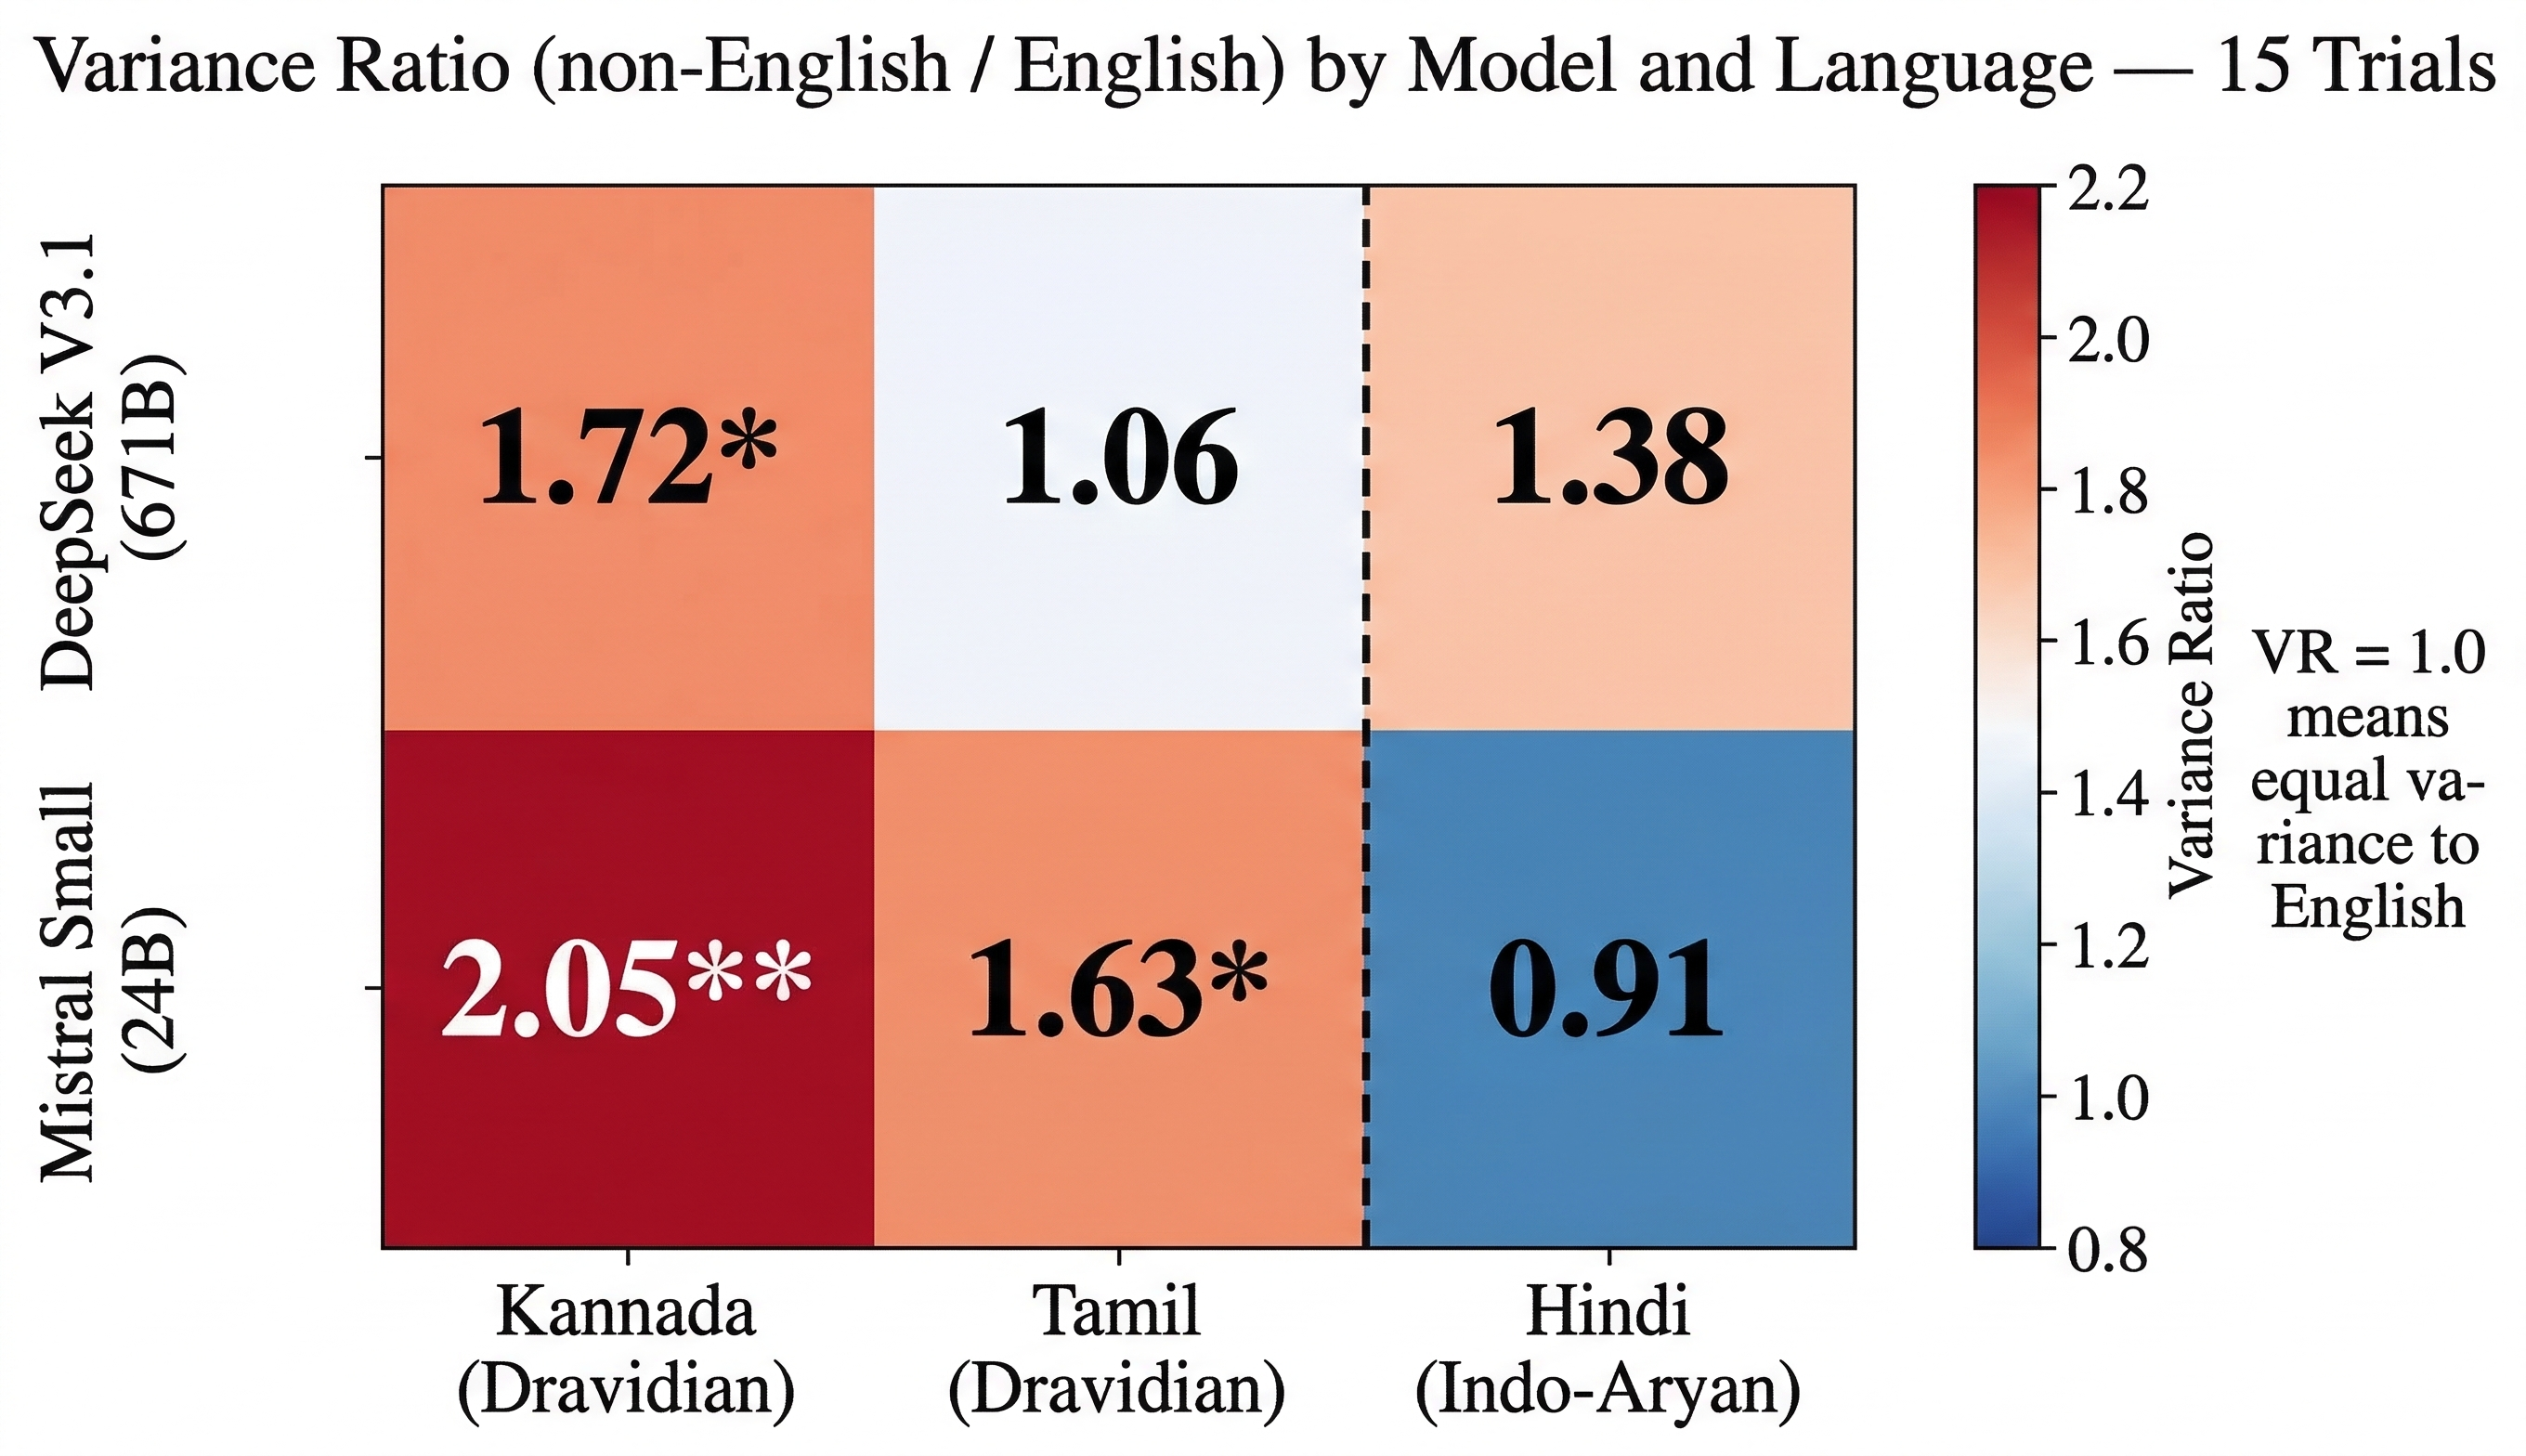
\includegraphics[width=0.75\textwidth]{figures/fig3_vr_heatmap.png}
\caption{Variance Ratio heatmap by model and language (15 trials). Kannada shows significant amplification in both models. Hindi shows no amplification despite equivalent EFI degradation. The dashed line separates Dravidian from Indo-Aryan languages.}
\label{fig:vr}
\end{figure}

\subsection{Code-Switching and Orthographic Corruption}

Analysis of the 600 raw responses reveals two additional failure modes invisible to embedding-based metrics:

\textbf{Code-switching:} When prompted in a non-English language, models frequently respond in English:

\begin{table}[H]
\centering
\caption{Percentage of responses beginning in English when prompted in the target non-English language (75 responses per cell).}
\label{tab:codeswitching}
\begin{tabular}{lccc}
\toprule
\textbf{Model} & \textbf{Kannada} & \textbf{Tamil} & \textbf{Hindi} \\
\midrule
DeepSeek V3.1   & 84\% & 40\% & 79\% \\
Mistral Small   & 45\% & 48\% & 59\% \\
\bottomrule
\end{tabular}
\end{table}

DeepSeek responds to Kannada medical prompts in English 84\% of the time (Figure~\ref{fig:codeswitching}). For a patient who reads only Kannada, this response is clinically useless regardless of its medical accuracy. The code-switching is scenario-dependent: for DeepSeek's Kannada responses, the preeclampsia scenario (S3) elicited 15/15 Kannada responses, while the diabetic foot scenario (S5) elicited 13/15 English responses --- indicating that the model's language choice depends on clinical content in unpredictable ways.

\begin{figure}[H]
\centering

\includegraphics[width=0.85\textwidth]{figures/fig4_codeswitching.png}
\caption{Language of response when prompted in non-English (75 responses per cell). DeepSeek responds in English 84\% of the time for Kannada prompts. The 50\% dashed line highlights that most model-language pairs default to English.}
\label{fig:codeswitching}
\end{figure}

\textbf{Orthographic corruption:} When Mistral does respond in Kannada, it misspells medical terms. The Kannada word for ``cough'' (\emph{kemmu}) appears as \emph{kachchassu}, \emph{kaammu}, \emph{keemu}, and \emph{kaasu} across different trials --- none of which are real Kannada words. A PHC doctor reading these responses would encounter unintelligible text for critical symptoms.

\textbf{Response fidelity} (fraction of response in target language):

\begin{table}[H]
\centering
\caption{Response fidelity: fraction of response content in the target non-English language (vs.\ English). Lower values indicate the model responds predominantly in English despite non-English prompts.}
\label{tab:fidelity}
\begin{tabular}{lcc}
\toprule
\textbf{Language} & \textbf{DeepSeek V3.1} & \textbf{Mistral Small} \\
\midrule
Kannada  & 0.531 & 0.051 \\
Tamil    & 0.406 & 0.205 \\
Hindi    & 0.350 & 0.073 \\
\bottomrule
\end{tabular}
\end{table}

Mistral's Kannada response fidelity is 5.1\% --- it responds almost entirely in English to Kannada medical prompts. Paradoxically, Mistral shows \emph{stronger} variance amplification for Kannada ($2.05\times$) than DeepSeek ($1.72\times$) despite its lower response fidelity. The model that fails more completely at language fidelity produces more variable outputs.

\subsection{The Encoding-to-Variance Pipeline}

Table~\ref{tab:pipeline} summarises the full degradation cascade from encoding to clinical output.

\begin{table}[H]
\centering
\caption{Summary: Encoding degradation propagates from embedding layer through generation to clinical output. Variance amplification shown for Kannada (the only language significant in both models).}
\label{tab:pipeline}
\begin{tabular}{llccc}
\toprule
\textbf{Layer} & \textbf{Metric} & \textbf{English} & \textbf{Kannada} & \textbf{Degradation} \\
\midrule
Embedding  & EFI (MiniLM)          & 1.000  & 0.099 & 90\% \\
Embedding  & EFI (MPNet)           & 1.000  & 0.125 & 87\% \\
Generation & Translation fidelity  & 1.000  & 0.52--0.86 & 14--48\% \\
Generation & Code-switching rate   & 0\%    & 45--84\%   & --- \\
Generation & Variance Ratio        & 1.00$\times$ & 1.72--2.05$\times$ & 72--105\%$\uparrow$ \\
\bottomrule
\end{tabular}
\end{table}

The pipeline reveals two key asymmetries. First, encoding degradation ($\sim$90\%) is far more severe than translation degradation (14--48\%), suggesting partial compensation during generation. Second, the generation layer introduces \emph{new} failure modes --- code-switching and orthographic corruption --- that are not predicted by encoding metrics alone. The model partially compensates for encoding loss in its generated content but cannot prevent the variance amplification or the language identity confusion.

% ================================================================
\section{Discussion}

\subsection{Shannon's Assumption Does Not Hold}

The $\sim$90\% EFI degradation demonstrated in Section~5.1 is not a marginal effect. It represents a near-total failure of encoding fidelity for non-English input. This failure persists across two embedding models of different dimensionalities (384D, 768D) and two LLMs of different scales (24B, 671B), indicating that it is not an artifact of any particular architecture.

Shannon's source coding theorem guarantees optimal coding \emph{given} encoding fidelity. When fidelity drops to $\sim$0.08, the theorem's preconditions are violated. The information bottleneck framework \citep{tishby2015} predicts that deep networks compress \emph{irrelevant} information while preserving task-relevant features. Our results show that for non-English medical input, the relevant information is being compressed because the model cannot distinguish it from noise.

\subsection{Coherent Misalignment as a Distinct Failure Mode}

Coherent Misalignment manifests in three distinct patterns in our data:

\begin{enumerate}
    \item \textbf{Translation corruption:} Mistral translates a Tamil sentence about a pregnant woman with hypertension into semantically unrelated content (cosine similarity = 0.21), while identifying the input language correctly.
    \item \textbf{Language identity confusion:} DeepSeek responds to Kannada medical prompts in English 84\% of the time --- producing medically accurate responses that the Kannada-speaking patient cannot read.
    \item \textbf{Orthographic corruption:} When Mistral does respond in Kannada, it generates misspelled medical terms (\emph{kachchassu}, \emph{kaammu} instead of \emph{kemmu} for ``cough'') --- unintelligible to the reader yet produced with full confidence formatting.
\end{enumerate}

None of these are hallucination --- the model is not inventing facts. None are deceptive alignment --- the model is not pursuing misaligned goals. They are Coherent Misalignment: the model operates faithfully on a degraded representation, producing output that appears correct from the outside but is clinically dangerous.

The code-switching failure is particularly insidious. A doctor in Karnataka who queries in Kannada and receives an English response might assume the system ``doesn't support Kannada'' and retype in English. But the degradation has already occurred at the encoding level --- the model's internal representation of the Kannada input is what generated the (English) response. The patient's symptoms, described in Kannada, may have been partially lost before generation began.

\subsection{$K \perp \text{Truth}$: Conservation Cannot Detect This}

Papers 2--6 showed that $K(\text{domain}) \approx \text{constant}$ across 14 models and 3 domains \citep{laxman2026b,laxman2026f}. $K$ measures the trade-off between context sensitivity ($\Delta$RCI) and output variance (Var\_Ratio) --- a structural property of how the model processes conversation.

A model with $\text{EFI} = 0.08$ and $\text{VR} = 2.05\times$ can show perfectly normal $K$. The conservation law holds because it measures \emph{variance structure}, not \emph{semantic content}. This is $K \perp \text{Truth}$: conservation is orthogonal to correctness.

The implication is stark: \textbf{no self-consistency metric can detect Coherent Misalignment}. A system that passes every internal consistency check --- normal $K$, normal $\Delta$RCI, normal Var\_Ratio structure --- may still be producing semantically degraded output for non-English input. External ground truth comparison is not optional; it is the only path to detection.

Figure~\ref{fig:pipeline} summarises the full failure cascade through Shannon's pipeline, showing how encoding degradation, variance amplification, and code-switching compound at successive stages while conservation metrics remain normal.

\begin{figure}[H]
\centering
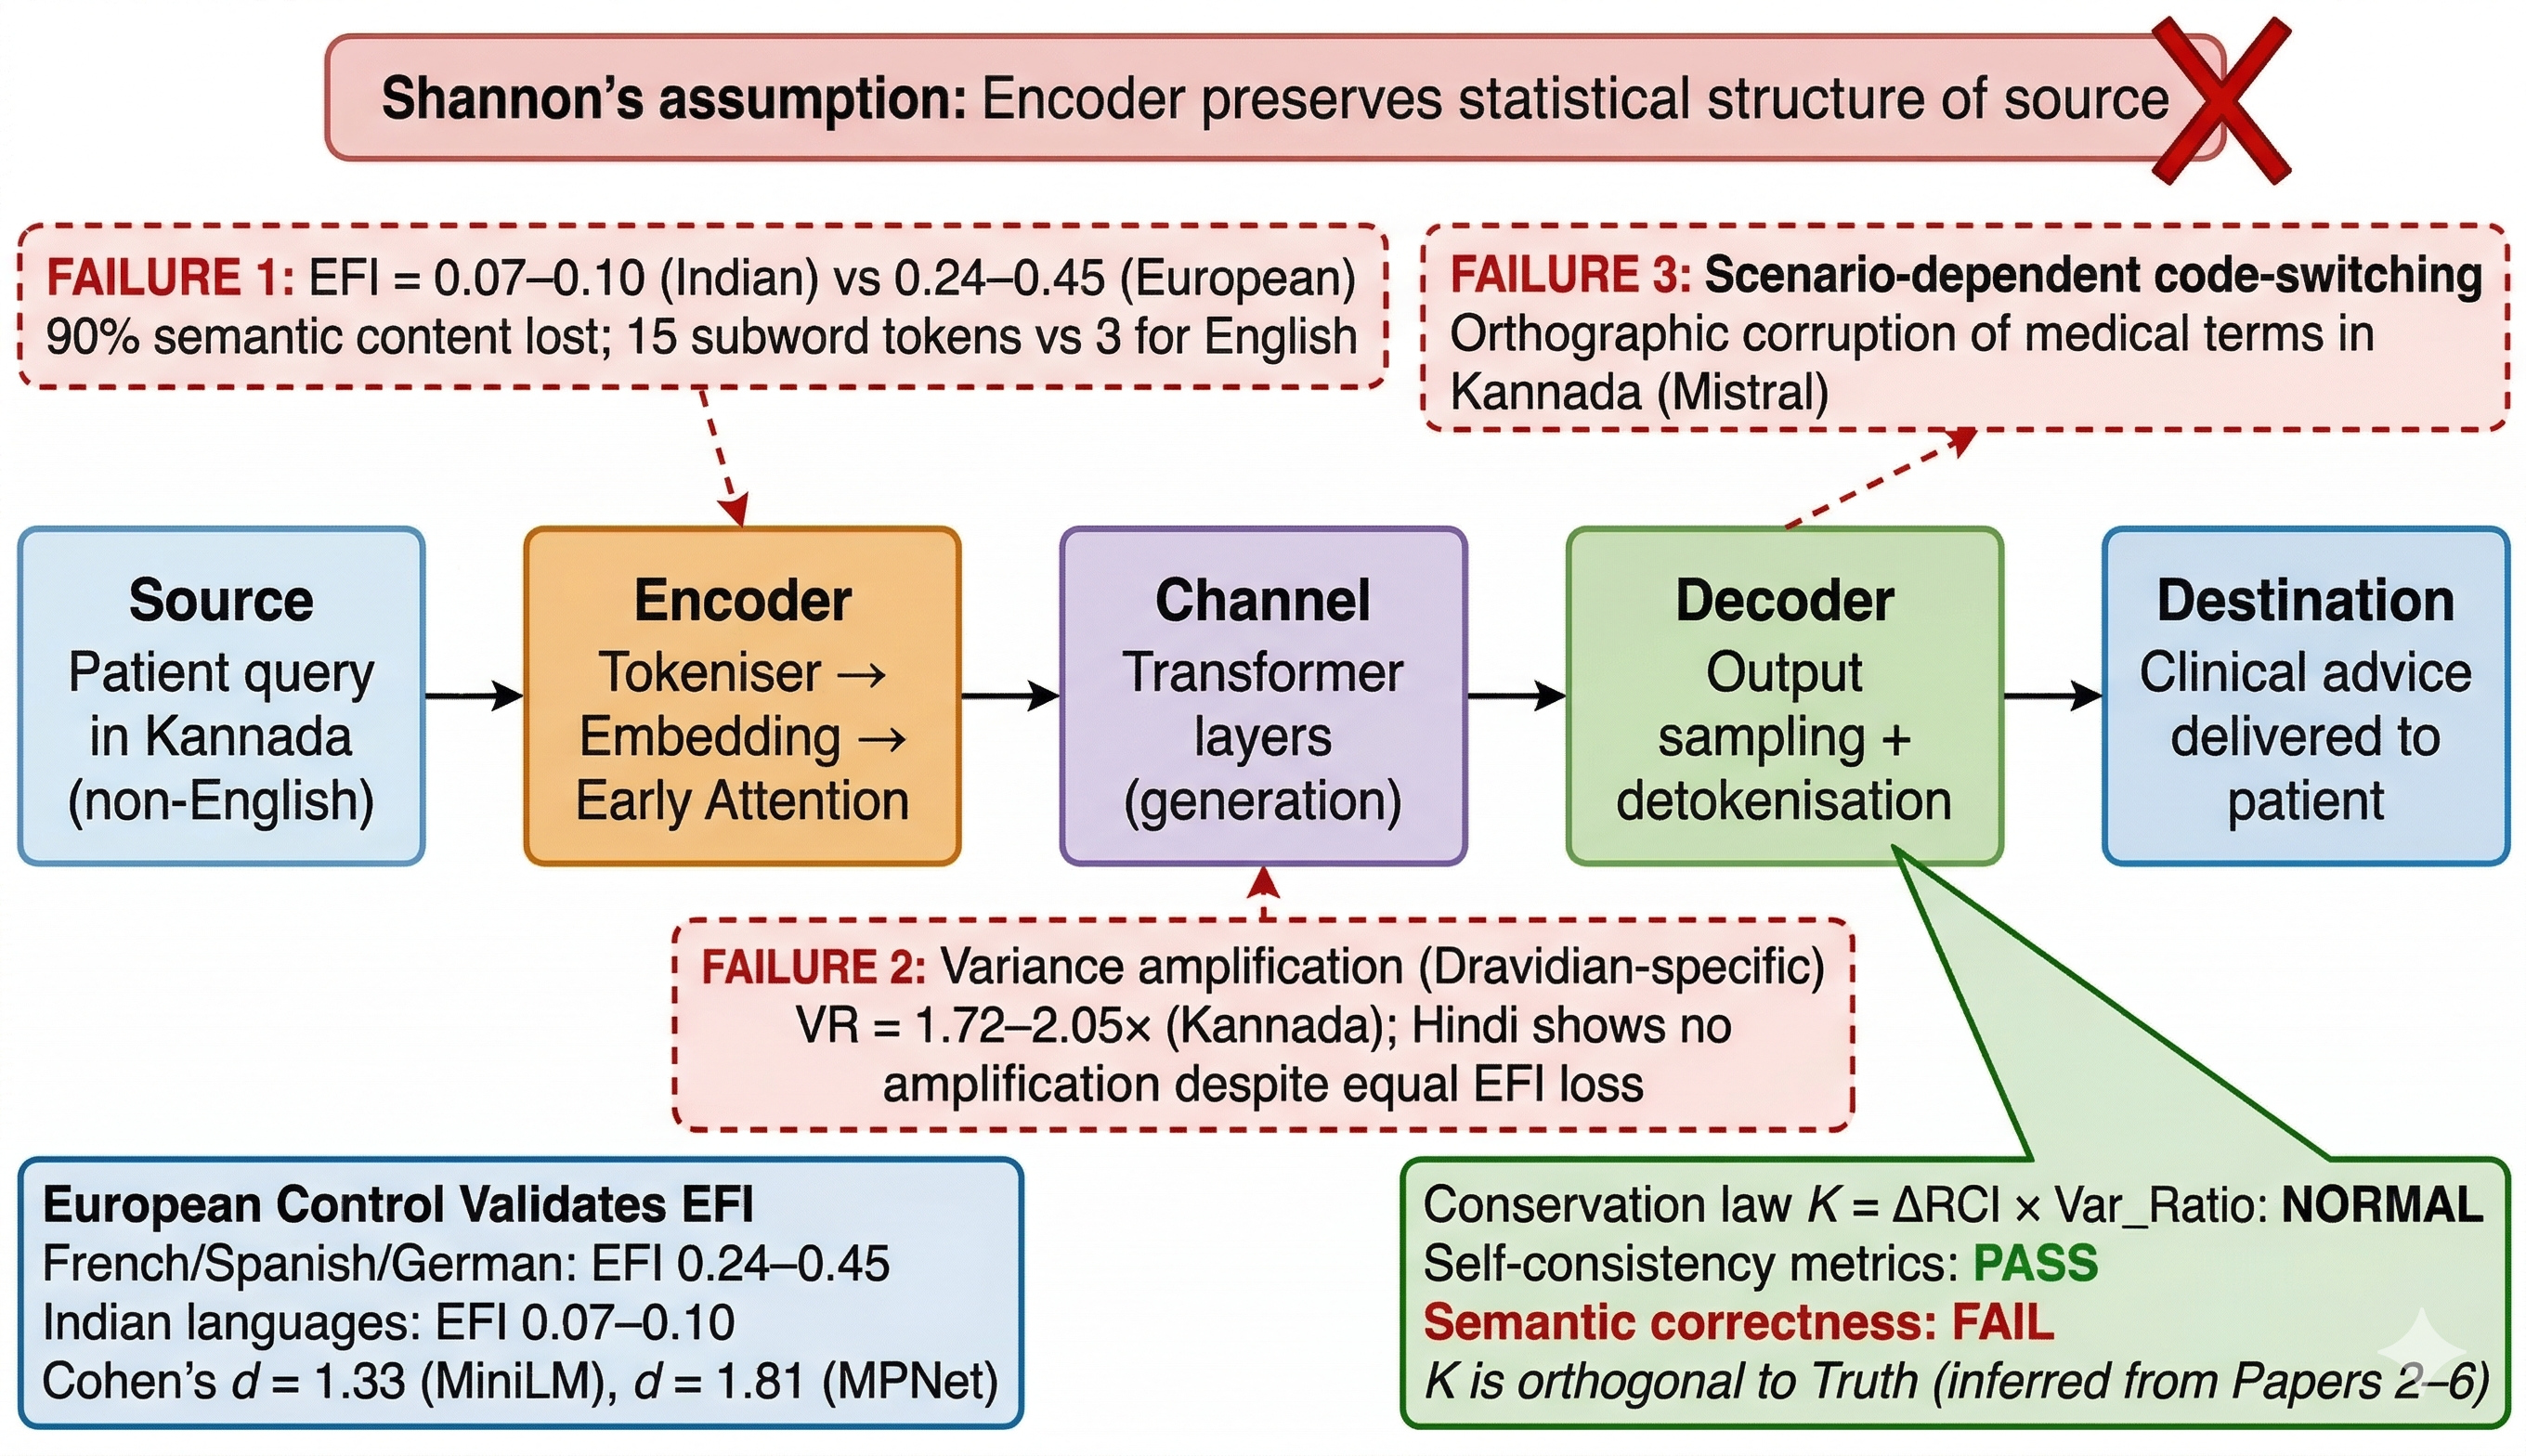
\includegraphics[width=0.95\textwidth]{figures/fig5_shannon_pipeline.png}
\caption{Shannon's communication pipeline applied to multilingual LLMs, with three failure points annotated. Shannon's encoding fidelity assumption (top, struck through) is violated at the encoder stage. Despite cascading failures through encoding, generation, and output, the conservation law $K = \Delta\text{RCI} \times \text{Var\_Ratio}$ remains normal --- $K \perp \text{Truth}$.}
\label{fig:pipeline}
\end{figure}

\subsection{The English Loanword Paradox}

The finding that complex medical sentences ($\text{EFI} = 0.14$ pooled, up to $0.17$ for Kannada) show higher encoding fidelity than simple sentences ($\text{EFI} = 0.08$) inverts the usual expectation that simpler input should be easier to encode. The explanation is English loanword anchoring: terms like ``ST elevation,'' ``D-dimer,'' and ``troponin'' are borrowed directly into Indian clinical practice without translation. In embedding space, these terms pull the representation toward the well-represented English region, partially rescuing fidelity.

This has a practical implication for clinical AI deployment: code-mixed queries (Kannada syntax with English medical terms) may be more reliable than either pure Kannada or literal Kannada translations of medical terminology. This is an observation, not a recommendation --- the fact that reliability depends on which language a doctor uses to ask the same question is itself evidence of a broken system.

\subsection{Clinical Implications}

A doctor querying an LLM in Kannada receives clinical advice that is:

\begin{itemize}
    \item Grammatically correct and fluent
    \item Confidently delivered with appropriate formatting
    \item In the wrong language 45--84\% of the time (English instead of Kannada)
    \item Up to $2.05\times$ more variable than the identical query in English
    \item Containing misspelled medical terms when in Kannada (Mistral)
\end{itemize}

The WHO's 2024 guidance on AI for health \citep{who2024} addresses ethical governance of large models but does not identify encoding fidelity as a failure mode. Current multilingual benchmarks \citep{xuan2025,adelani2025} measure task accuracy across languages but not the encoding-variance pipeline that produces unreliable clinical advice.

Over 1.5 billion people worldwide speak languages where LLM encoding fidelity is likely degraded. For these populations, the promise of AI-assisted healthcare carries a hidden cost: the system appears to work, passes all internal consistency checks, and produces output that looks correct --- but is less reliable than the same system operating in English.

\subsection{Limitations}

Five limitations should be noted:

\begin{enumerate}
    \item \textbf{Proxy metric:} EFI\textsubscript{proxy} measures embedding cosine similarity, not the true mutual information $I(X; \hat{X})$. The relationship between the proxy and the theoretical quantity requires formal characterisation.
    \item \textbf{Sample size:} Fifteen clinical sentences (5 per complexity level) is sufficient for detecting the large effects reported here but insufficient for fine-grained analysis of sentence-level factors.
    \item \textbf{Language coverage:} Three Indian languages were tested. Extension to African, Southeast Asian, and other language families is needed to establish universality.
    \item \textbf{No direct clinical harm measurement:} We demonstrate degraded encoding and amplified variance, not patient outcomes. A prospective clinical validation study is required.
    \item \textbf{Causal mechanism:} The variance amplification is Dravidian-specific despite universal EFI degradation, indicating that the simple relationship $\text{VR} \propto 1/\text{EFI}$ does not hold. Training data representation likely mediates the encoding-to-variance pathway, but the precise mechanism requires further investigation.
    \item \textbf{Two models:} Experiment~5 uses two LLMs. While the Kannada effect replicates across both, extension to more models is needed to confirm the Dravidian specificity.
\end{enumerate}

% ================================================================
\section{Conclusion}

Shannon's Mathematical Theory of Communication assumed encoding fidelity. LLMs violate this assumption systematically for non-English languages, producing Coherent Misalignment --- outputs that are internally consistent but semantically degraded. Using the Encoding Fidelity Index, we measured $\sim$90\% encoding degradation for Kannada, Tamil, and Hindi. The downstream consequences are language-specific: Kannada shows $1.72$--$2.05\times$ variance amplification (replicated across both models), pervasive code-switching (84\% English responses to Kannada prompts), and orthographic corruption of medical terms. Hindi, despite equivalent EFI degradation, shows no variance amplification --- revealing that training data representation, not encoding fidelity alone, determines clinical reliability.

The conservation law $K(\text{domain})$ holds normally throughout --- $K \perp \text{Truth}$ --- meaning no self-consistency metric can detect this failure. The system knows what fits, but not what is true.

Clinical AI deployment in linguistically diverse populations requires external truth anchoring, not just internal consistency checks. The encoding fidelity gap is a new failure mode that extends Shannon's original model. For the 50 million Kannada speakers and 1.5 billion non-English speakers worldwide, measurement of encoding fidelity must precede deployment.

% ================================================================
\section{Future Work}

\begin{enumerate}
    \item \textbf{Cross-linguistic extension:} Measure EFI across African (Yoruba, Swahili), Southeast Asian (Bahasa, Thai), and European (Romanian, Hungarian) languages using the same protocol.
    \item \textbf{EFI-aware tokenisation:} Develop tokenisers that equalise encoding fidelity across languages, guided by EFI as an optimisation target.
    \item \textbf{Prospective clinical study:} Deploy LLMs in a PHC setting and measure real-world clinical error rates as a function of query language.
    \item \textbf{Formal EFI--VR derivation:} Derive the relationship between encoding fidelity and variance amplification from information-theoretic first principles.
    \item \textbf{Safety framework integration:} Incorporate EFI into LLM safety evaluation frameworks alongside $\Delta$RCI, VRI, and $K$.
\end{enumerate}

% ================================================================
\section*{Acknowledgements}

This research was conducted entirely at Primary Health Centre Manchi, Karnataka, India, using personal resources. No external funding was received. The clinical perspective in this paper comes from daily practice --- treating patients in Kannada who deserve the same quality of AI-assisted care as English speakers.

% ================================================================
\bibliographystyle{plainnat}

\begin{thebibliography}{27}

\bibitem[Adelani et~al.(2025)]{adelani2025}
Adelani, D.~I., Ojo, J., Azime, I.~A., et~al. (2025).
\newblock IrokoBench: A new benchmark for African languages in the age of large language models.
\newblock \emph{Proceedings of NAACL 2025}, 2732--2757. Outstanding Paper Award.
\newblock arXiv: 2406.03368.

\bibitem[Ali et~al.(2024)]{ali2024}
Ali, M., Fromm, M., Thellmann, K., et~al. (2024).
\newblock Tokenizer choice for {LLM} training: Negligible or crucial?
\newblock \emph{Findings of NAACL 2024}, 3907--3924.
\newblock arXiv: 2310.08754.

\bibitem[Alonso et~al.(2024)]{alonso2024}
Alonso, I., Oronoz, M., \& Agerri, R. (2024).
\newblock {MedExpQA}: Multilingual benchmarking of large language models for medical question answering.
\newblock \emph{Artificial Intelligence in Medicine}, 155, 102938.
\newblock arXiv: 2404.05590.

\bibitem[Ardoin et~al.(2025)]{ardoin2025}
Ardoin, T., Cai, Y., \& Wunder, G. (2025).
\newblock Where confabulation lives: Latent feature discovery in {LLMs}.
\newblock \emph{Proceedings of EMNLP 2025}, 29813--29837.

\bibitem[Asgari et~al.(2025)]{asgari2025}
Asgari, E., Montana-Brown, N., Dubois, M., et~al. (2025).
\newblock A framework to assess clinical safety and hallucination rates of {LLMs} for medical text summarisation.
\newblock \emph{npj Digital Medicine}, 8(1), 274.
\newblock DOI: 10.1038/s41746-025-01670-7.

\bibitem[Chakravarthi et~al.(2022)]{chakravarthi2022}
Chakravarthi, B.~R., Priyadharshini, R., Muralidaran, V., et~al. (2022).
\newblock {DravidianCodeMix}: Sentiment analysis and offensive language identification dataset for {D}ravidian languages in code-mixed text.
\newblock \emph{Language Resources and Evaluation}.
\newblock DOI: 10.1007/s10579-022-09583-7.

\bibitem[Del\'{e}tang et~al.(2024)]{deletang2024}
Del\'{e}tang, G., Ruoss, A., Duquenne, P.-A., et~al. (2024).
\newblock Language modeling is compression.
\newblock \emph{ICLR 2024}.
\newblock arXiv: 2309.10668.

\bibitem[Hammerl et~al.(2024)]{hammerl2024}
Hammerl, K., Libovick\'{y}, J., \& Fraser, A. (2024).
\newblock Understanding cross-lingual alignment --- a survey.
\newblock \emph{Findings of ACL 2024}, 10922--10943.
\newblock arXiv: 2404.06228.

\bibitem[Hubinger et~al.(2019)]{hubinger2019}
Hubinger, E., van Merwijk, C., Mikulik, V., Skalse, J., \& Garrabrant, S. (2019).
\newblock Risks from learned optimization in advanced machine learning systems.
\newblock arXiv: 1906.01820.

\bibitem[Laxman(2026a)]{laxman2026a}
Laxman, M.~M. (2026a).
\newblock Context curves behavior: Measuring {AI} relational dynamics with {$\Delta$RCI}.
\newblock \emph{Preprints.org}, 202601.1881.

\bibitem[Laxman(2026b)]{laxman2026b}
Laxman, M.~M. (2026b).
\newblock Scaling context sensitivity: Standardized benchmark across 25 {LLM}-domain configurations.
\newblock \emph{Preprints.org}, 202602.1114.

\bibitem[Laxman(2026c)]{laxman2026c}
Laxman, M.~M. (2026c).
\newblock Domain-specific temporal dynamics of context sensitivity in large language models.
\newblock \emph{Preprints.org}, 202602.1674.

\bibitem[Laxman(2026d)]{laxman2026d}
Laxman, M.~M. (2026d).
\newblock Engagement as entanglement: Variance signatures of bidirectional context coupling in large language models.
\newblock \emph{Preprints.org}, DOI: 10.20944/preprints202603.0055.v1.

\bibitem[Laxman(2026e)]{laxman2026e}
Laxman, M.~M. (2026e).
\newblock Stochastic incompleteness: A predictability taxonomy for clinical {AI} deployment.
\newblock \emph{Preprints.org}, DOI: 10.20944/preprints202602.2034.v1.

\bibitem[Laxman(2026f)]{laxman2026f}
Laxman, M.~M. (2026f).
\newblock Conservation constraint across three domains.
\newblock \emph{In preparation}.

\bibitem[Laxman(2026g)]{laxman2026g}
Laxman, M.~M. (2026g).
\newblock The structure and trajectory of context sensitivity in {LLMs}: Content-order decomposition and variance dissociation.
\newblock \emph{Preprints.org}, DOI: 10.20944/preprints202603.1116.v1.

\bibitem[Lundin et~al.(2025)]{lundin2025}
Lundin, J.~M., Zhang, A., Karim, N., et~al. (2025).
\newblock The token tax: Systematic bias in multilingual tokenization.
\newblock arXiv: 2509.05486.

\bibitem[Pallucchini et~al.(2025)]{pallucchini2025}
Pallucchini, F., Malandri, L., Mercorio, F., \& Mezzanzanica, M. (2025).
\newblock Lost in alignment: A survey on cross-lingual alignment methods for contextualized representation.
\newblock \emph{ACM Computing Surveys}, 58(5).
\newblock DOI: 10.1145/3764112.

\bibitem[Peng \& S{\o}gaard(2024)]{peng2024}
Peng, Q. \& S{\o}gaard, A. (2024).
\newblock Concept space alignment in multilingual {LLMs}.
\newblock \emph{Proceedings of EMNLP 2024}, 5511--5526.

\bibitem[Petrov et~al.(2023)]{petrov2023}
Petrov, A., La~Malfa, E., Torr, P.~H.~S., \& Bibi, A. (2023).
\newblock Language model tokenizers introduce unfairness between languages.
\newblock \emph{NeurIPS 2023}.
\newblock arXiv: 2305.15425.

\bibitem[Qiu et~al.(2024)]{qiu2024}
Qiu, P., Wu, C., Zhang, X., et~al. (2024).
\newblock Towards building multilingual language model for medicine.
\newblock \emph{Nature Communications}, 15, 8384.
\newblock DOI: 10.1038/s41467-024-52417-z.

\bibitem[Rust et~al.(2021)]{rust2021}
Rust, P., Pfeiffer, J., Vuli\'{c}, I., Ruder, S., \& Gurevych, I. (2021).
\newblock How good is your tokenizer? {O}n the monolingual performance of multilingual language models.
\newblock \emph{Proceedings of ACL-IJCNLP 2021}, 3118--3135.
\newblock arXiv: 2012.15613.

\bibitem[Shannon(1948)]{shannon1948}
Shannon, C.~E. (1948).
\newblock A mathematical theory of communication.
\newblock \emph{Bell System Technical Journal}, 27(3), 379--423; 27(4), 623--656.
\newblock DOI: 10.1002/j.1538-7305.1948.tb01338.x.

\bibitem[Shwartz-Ziv \& Tishby(2017)]{shwartzziv2017}
Shwartz-Ziv, R. \& Tishby, N. (2017).
\newblock Opening the black box of deep neural networks via information.
\newblock arXiv: 1703.00810.

\bibitem[Tishby \& Zaslavsky(2015)]{tishby2015}
Tishby, N. \& Zaslavsky, N. (2015).
\newblock Deep learning and the information bottleneck principle.
\newblock \emph{IEEE Information Theory Workshop (ITW)}, 1--5.
\newblock DOI: 10.1109/ITW.2015.7133169.

\bibitem[{WHO}(2024)]{who2024}
{World Health Organization} (2024).
\newblock \emph{Ethics and Governance of Artificial Intelligence for Health: Guidance on Large Multi-Modal Models}.
\newblock Geneva: WHO.
\newblock ISBN: 978-92-4-008475-9.

\bibitem[Xuan et~al.(2025)]{xuan2025}
Xuan, W., Yang, R., Qi, H., et~al. (2025).
\newblock {MMLU-ProX}: A multilingual benchmark for advanced large language model evaluation.
\newblock \emph{Proceedings of EMNLP 2025}.
\newblock arXiv: 2503.10497.

\end{thebibliography}

\end{document}
